\documentclass[11pt]{article}
\usepackage[letterpaper,landscape,margin=0.65in]{geometry}
\usepackage{booktabs,graphicx}
\setlength{\parindent}{0pt}
\setlength{\parskip}{6pt}
\begin{document}
\begin{center}\Large\textbf{Communication proxies and the individual rationality gradient}\end{center}
\textbf{Finding.} These splits do not support a stronger minimum-CCEI association with group CCEI when communication
is presumed easier. Point estimates are smaller at endline, among friends, and in higher-math groups. The friendship
differences are statistically clearer; the wave and math differences in minimum-CCEI slopes are not.

\begin{center}\small
\begin{tabular}{lrrrrr}\toprule
Comparison & Group CCEI: $\beta_{\min}$ & Difference $p$ & CEIV: $\beta_{\min}$ & Difference $p$ & Selectivity $p$\\
& Lower $\to$ higher proxy & & Lower $\to$ higher proxy & & CCEI minus CEIV\\\midrule
Baseline $\to$ endline & 0.269 $\to$ 0.207 & 0.445 & 0.077 $\to$ 0.099 & 0.732 & 0.172\\
No $\to$ any nomination & 0.311 $\to$ -0.010 & $<0.001$ & 0.120 $\to$ -0.056 & 0.018 & 0.002\\
Pair math: below $\to$ at/above median & 0.294 $\to$ 0.168 & 0.174 & 0.131 $\to$ 0.033 & 0.204 & 0.719\\
Less-rational math: below $\to$ at/above & 0.285 $\to$ 0.176 & 0.213 & 0.099 $\to$ 0.045 & 0.446 & 0.343\\
\bottomrule\end{tabular}\end{center}
\small
\textit{Specification:} Table 5 column (3): both individual CCEIs, student/personality, friendship/network, and
corner/midpoint-share controls, with class fixed effects and class-clustered standard errors. Risk-aversion controls
are excluded. Coefficients are per one-unit increase in individual CCEI; multiply by 0.1 for a 0.1 increase. Comparisons
are descriptive and unadjusted for multiple testing. Math cutoffs are wave-specific; median ties enter the higher bin.

\textbf{Tests of the proposed channel.} Comparing significance across outcomes is insufficient. ``Selectivity'' tests
whether the moderator changes the minimum-CCEI coefficient differently for group CCEI and CEIV, by fitting the same
model to CCEI minus CEIV. The binary friendship contrast is a larger decline for group CCEI ($\Delta=-0.146$, $p=0.002$),
the opposite direction to the proposed complementarity. This selective decline is less precisely estimated when
one-sided and mutual friendships have separate slopes and controls. Adding wave fixed effects preserves the main direction.

\textbf{Another pattern.} Maximum individual CCEI has a larger CEIV coefficient in higher-math groups: a slope difference
of 0.551 ($p<0.001$) for pair-average math and 0.452 ($p=0.004$) for the less rational member's math. This is a different
pattern from the proposed minimum-CCEI channel. The cross-outcome tests do not establish that this moderation is
larger for CEIV than for CCEI.

\textbf{Implication for the draft.} Point (2) should remain an open hypothesis. An alternative possibility is that easier
coordination substitutes for the less rational member's rationality, but these observational proxies do not identify that
mechanism. The survey evidence supports perceived similarity more clearly than shared or own influence. Group CCEI
does not identify stable weights, CEIV does not identify turn-taking, and the prior RA-gap split weakens rather than
fully excludes a risk-preference explanation. A normative reason to prefer stable weights requires an additional argument.
\clearpage
\begin{center}\Large\textbf{Baseline versus endline}\end{center}
\small
Split the same 652 pairs into baseline and endline (652 pair-waves each). Endline is a proxy for additional experience, not a randomized communication treatment.
\begin{center}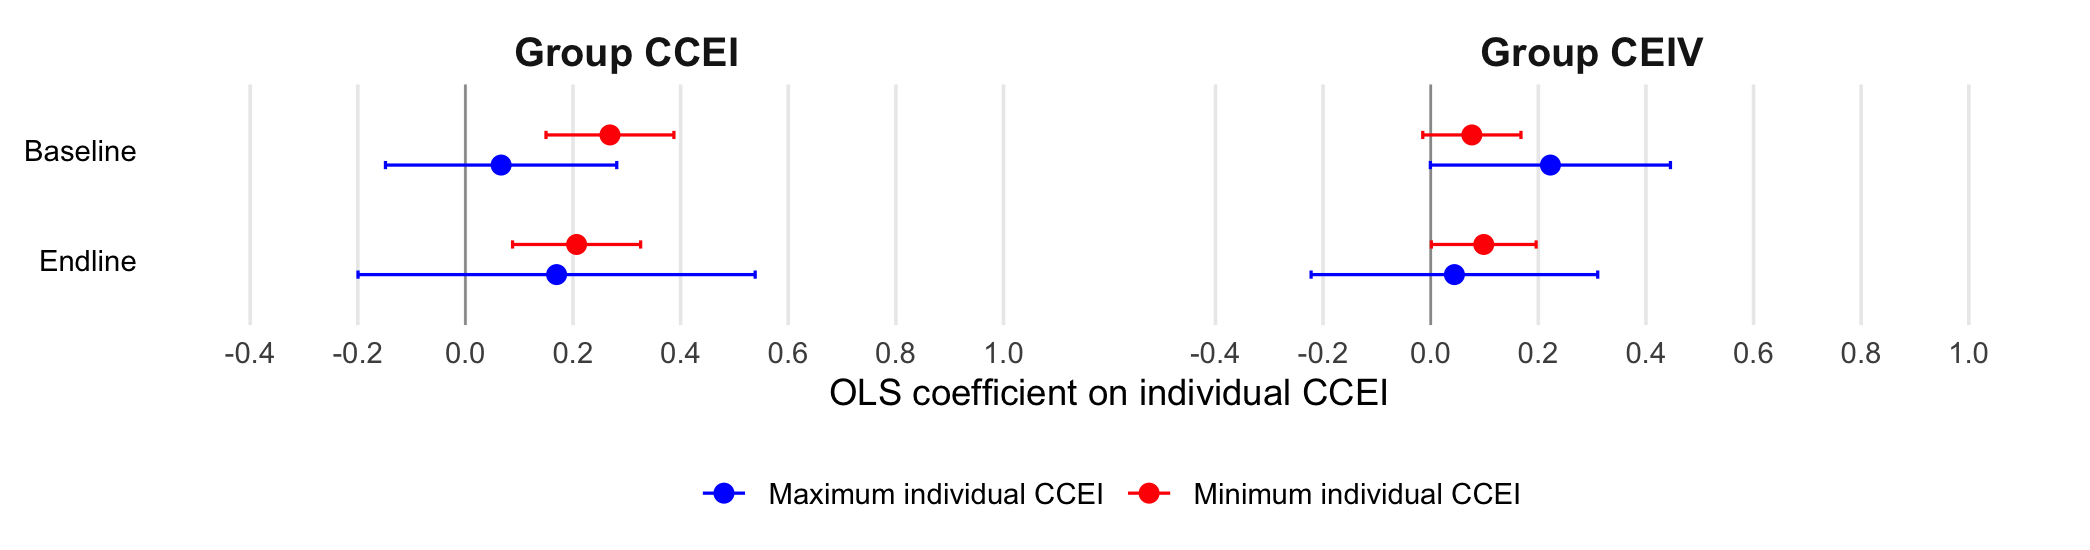
\includegraphics[width=\textwidth]{wave_coefficients.png}\end{center}
\begin{center}\begin{tabular}{lrrrrrr}\toprule
Sample & Fitted $N$ & Classes & CCEI: maximum & CCEI: minimum & CEIV: maximum & CEIV: minimum\\\midrule
Eligible pooled reference & 1304 & 64 & 0.131 (0.095) & 0.235 (0.045) & 0.176 (0.094) & 0.086 (0.035)\\
Baseline & 652 & 64 & 0.066 (0.108) & 0.269 (0.059) & 0.222 (0.112) & 0.077 (0.046)\\
Endline & 652 & 64 & 0.169 (0.185) & 0.207 (0.060) & 0.044 (0.133) & 0.099 (0.049)\\
\bottomrule\end{tabular}\end{center}
\begin{center}\begin{tabular}{llrrr}\toprule
Higher minus lower group & Individual CCEI & $\Delta$ group CCEI ($p$) & $\Delta$ CEIV ($p$) & $\Delta$(CCEI--CEIV) ($p$)\\\midrule
Higher minus lower & Minimum & -0.062 (0.445) & 0.022 (0.732) & -0.084 (0.172)\\
Higher minus lower & Maximum & 0.103 (0.642) & -0.178 (0.316) & 0.282 (0.110)\\
\bottomrule\end{tabular}\end{center}
\textbf{Reading the pattern.} The minimum-CCEI association is smaller at endline, with no clear slope difference for either outcome. The endline group CCEI level and share equal to one are higher, so the split also changes outcome distributions and available room for improvement.
\textit{Support check:} Mean minimum individual CCEI by subgroup: 0.838, 0.882; share of group CCEI equal to one: 39.1\%, 51.2\%. These describe eligible samples before singleton exclusions.
\textit{Notes:} Class-clustered SEs are in parentheses; 95\% intervals are plotted. Differences use pooled OLS fully interacting subgroup membership with both CCEIs, all controls, and class effects, accounting for shared classes. Pooled references use eligible samples; separate fits drop observations in singleton classes. Eligible counts are in the introduction; fitted counts are in the table.
\clearpage
\begin{center}\Large\textbf{Dyadic friendship: three nomination categories}\end{center}
\small
Friendship uses directed nominations: none, one-sided, or mutual. Eligible counts are 912/225/167 pair-waves; 167 pairs change category between waves. The split is contemporaneous rather than fixed at baseline.
\begin{center}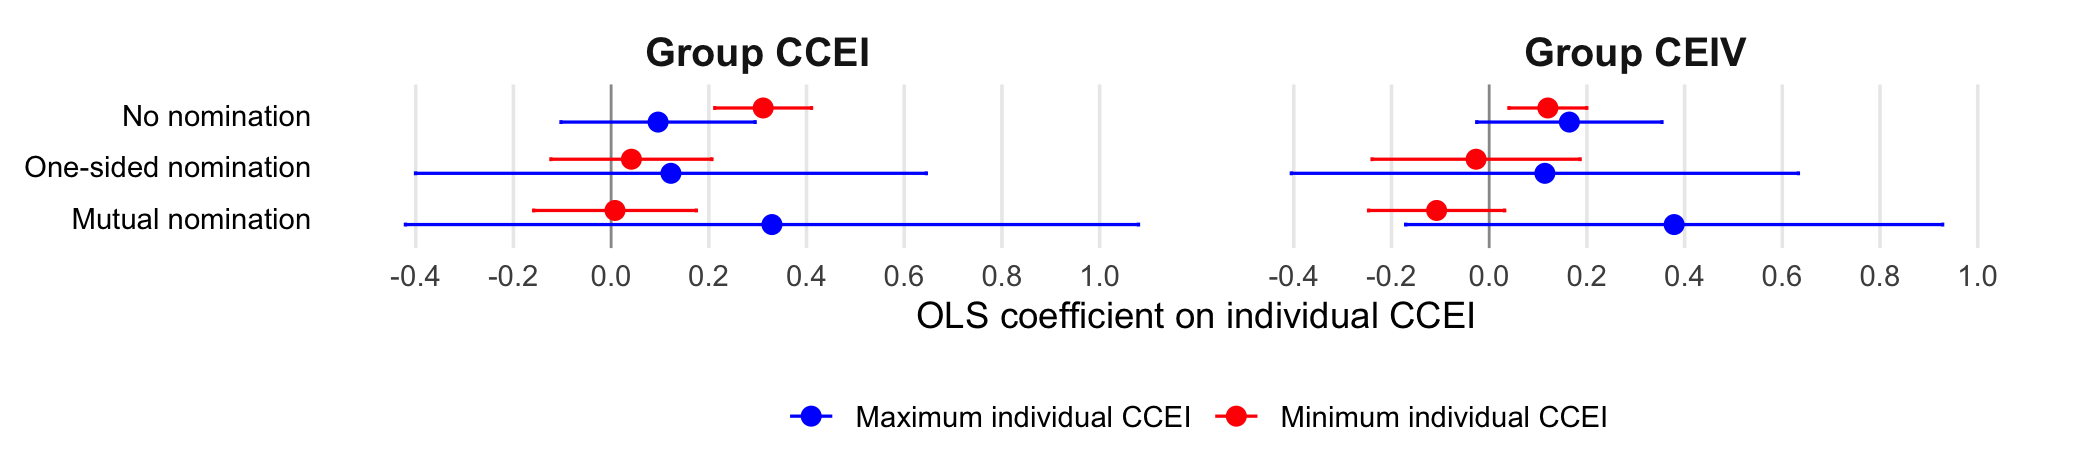
\includegraphics[width=\textwidth]{friend_coefficients.png}\end{center}
\begin{center}\begin{tabular}{lrrrrrr}\toprule
Sample & Fitted $N$ & Classes & CCEI: maximum & CCEI: minimum & CEIV: maximum & CEIV: minimum\\\midrule
Eligible pooled reference & 1304 & 64 & 0.131 (0.095) & 0.235 (0.045) & 0.176 (0.094) & 0.086 (0.035)\\
No nomination & 912 & 64 & 0.096 (0.099) & 0.311 (0.050) & 0.164 (0.095) & 0.120 (0.040)\\
One-sided nomination & 213 & 46 & 0.122 (0.260) & 0.042 (0.082) & 0.114 (0.258) & -0.027 (0.106)\\
Mutual nomination & 159 & 46 & 0.329 (0.373) & 0.008 (0.083) & 0.379 (0.273) & -0.108 (0.069)\\
\bottomrule\end{tabular}\end{center}
\begin{center}\begin{tabular}{llrrr}\toprule
Higher minus lower group & Individual CCEI & $\Delta$ group CCEI ($p$) & $\Delta$ CEIV ($p$) & $\Delta$(CCEI--CEIV) ($p$)\\\midrule
1 minus 0 & Minimum & -0.270 (0.008) & -0.147 (0.203) & -0.123 (0.114)\\
2 minus 0 & Minimum & -0.303 (0.004) & -0.228 (0.010) & -0.076 (0.300)\\
2 minus 1 & Minimum & -0.034 (0.803) & -0.081 (0.557) & 0.047 (0.632)\\
\addlinespace\multicolumn{5}{l}{\textit{Wave-fixed-effects check: minimum CCEI}}\\
1 minus 0 & Minimum & -0.289 (0.005) & -0.146 (0.218) & -0.143 (0.088)\\
2 minus 0 & Minimum & -0.304 (0.004) & -0.226 (0.011) & -0.078 (0.285)\\
\bottomrule\end{tabular}\end{center}
Friendship coding in the contrast table: 0=no nomination, 1=one-sided, 2=mutual.
\textbf{Reading the pattern.} The minimum-CCEI coefficient on group CCEI is smaller in both friendship groups. The CEIV coefficient is also smaller, particularly for mutual nominations. Neither separate friendship contrast establishes CCEI-specific moderation; a difference in within-model significance is not such a test.
\textit{Support check:} Mean minimum individual CCEI by subgroup: 0.856, 0.869, 0.869; share of group CCEI equal to one: 43.9\%, 51.6\%, 43.7\%. These describe eligible samples before singleton exclusions.
\textit{Notes:} Class-clustered SEs are in parentheses; 95\% intervals are plotted. Differences use pooled OLS fully interacting subgroup membership with both CCEIs, all controls, and class effects, accounting for shared classes. Pooled references use eligible samples; separate fits drop observations in singleton classes. Eligible counts are in the introduction; fitted counts are in the table.
\clearpage
\begin{center}\Large\textbf{Pair-average math score}\end{center}
\small
Compute the average of both members' observed math scores (0--5). Exclude 13 pair-waves with at least one missing score. The median is 2.5 at baseline and 3.0 at endline; high means at or above that wave's median. Eligible low/high counts are 530/761. Median ties number 111/123 at baseline/endline and are retained in the high group.
\begin{center}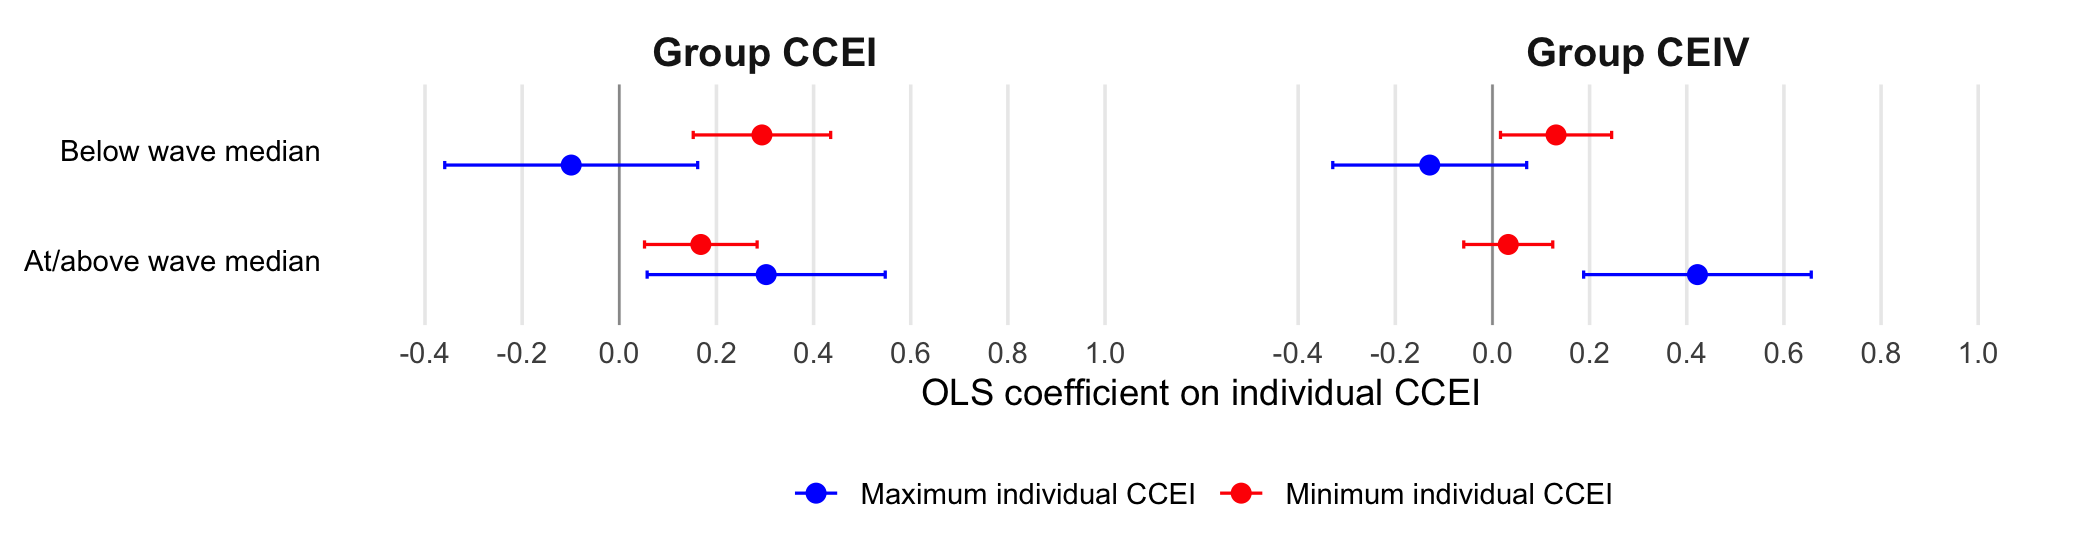
\includegraphics[width=\textwidth]{math_pair_coefficients.png}\end{center}
\begin{center}\begin{tabular}{lrrrrrr}\toprule
Sample & Fitted $N$ & Classes & CCEI: maximum & CCEI: minimum & CEIV: maximum & CEIV: minimum\\\midrule
Eligible pooled reference & 1291 & 64 & 0.134 (0.096) & 0.235 (0.045) & 0.179 (0.094) & 0.088 (0.035)\\
Below wave median & 527 & 59 & -0.099 (0.130) & 0.294 (0.071) & -0.129 (0.100) & 0.131 (0.057)\\
At/above wave median & 761 & 64 & 0.302 (0.123) & 0.168 (0.058) & 0.422 (0.117) & 0.033 (0.046)\\
\bottomrule\end{tabular}\end{center}
\begin{center}\begin{tabular}{llrrr}\toprule
Higher minus lower group & Individual CCEI & $\Delta$ group CCEI ($p$) & $\Delta$ CEIV ($p$) & $\Delta$(CCEI--CEIV) ($p$)\\\midrule
Higher minus lower & Minimum & -0.126 (0.174) & -0.098 (0.204) & -0.027 (0.719)\\
Higher minus lower & Maximum & 0.401 (0.037) & 0.551 ($<0.001$) & -0.150 (0.383)\\
\addlinespace\multicolumn{5}{l}{\textit{Wave-fixed-effects check: minimum CCEI}}\\
Higher minus lower & Minimum & -0.115 (0.210) & -0.099 (0.204) & -0.017 (0.828)\\
\bottomrule\end{tabular}\end{center}
\textbf{Reading the pattern.} Minimum-CCEI point estimates are smaller in the higher-math group, but their differences are imprecise. Maximum-CCEI coefficients are larger for both outcomes, with a clearer CEIV difference. These findings do not support the predicted stronger minimum-CCEI gradient.
\textit{Support check:} Mean minimum individual CCEI by subgroup: 0.852, 0.867; share of group CCEI equal to one: 43.8\%, 46.3\%. These describe eligible samples before singleton exclusions.
\textit{Notes:} Class-clustered SEs are in parentheses; 95\% intervals are plotted. Differences use pooled OLS fully interacting subgroup membership with both CCEIs, all controls, and class effects, accounting for shared classes. Pooled references use eligible samples; separate fits drop observations in singleton classes. Eligible counts are in the introduction; fitted counts are in the table.
\clearpage
\begin{center}\Large\textbf{Math score of the less rational member}\end{center}
\small
Select the member with strictly lower individual CCEI in each pair and wave. Exclude 199 CCEI-tied pair-waves and 11 additional pair-waves missing the selected member's math score. The math median is 3 in both waves; low is below 3, high is at least 3. Eligible low/high counts are 522/572 (1,094 total). Median ties are 116/104 at baseline/endline. The selected member can change across waves.
\begin{center}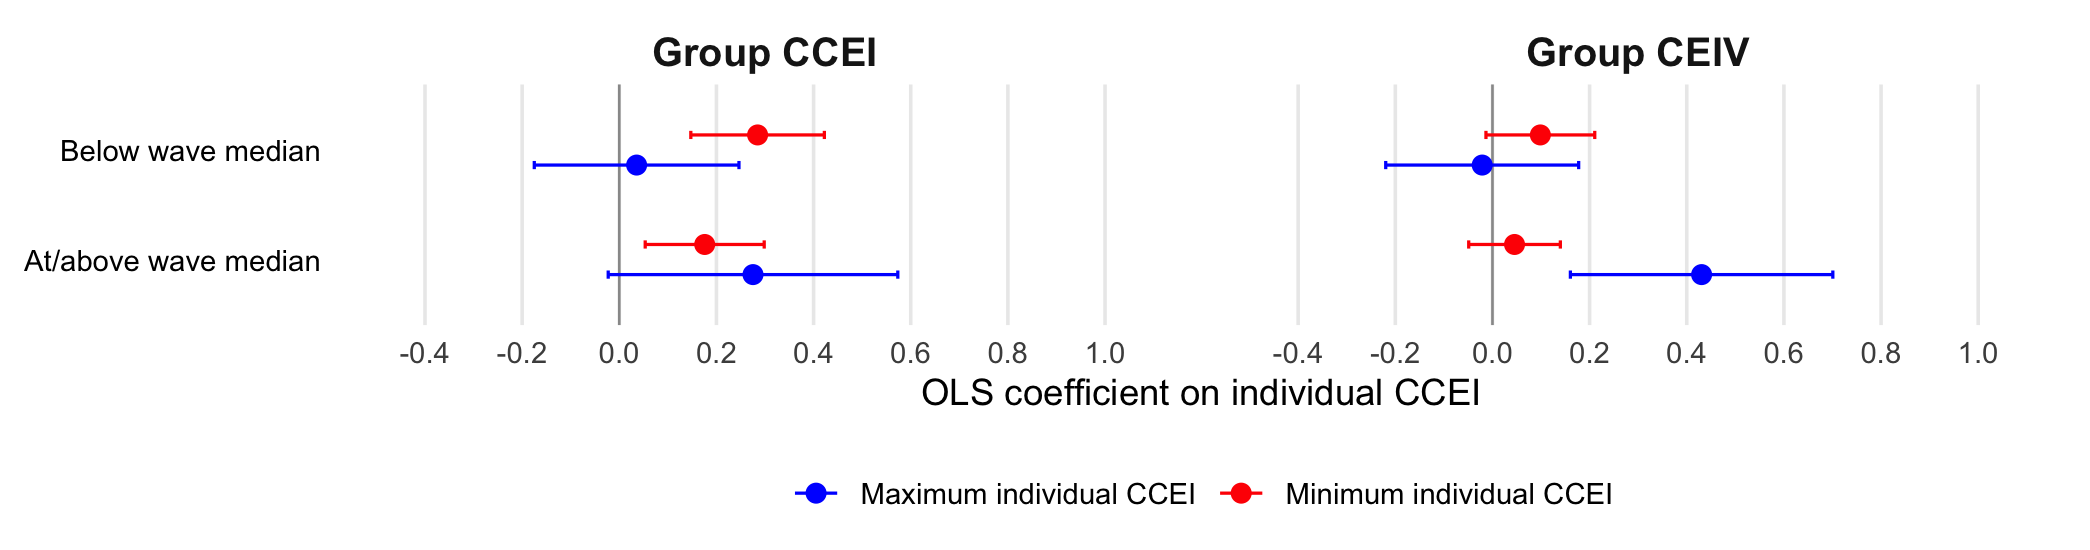
\includegraphics[width=\textwidth]{math_less_coefficients.png}\end{center}
\begin{center}\begin{tabular}{lrrrrrr}\toprule
Sample & Fitted $N$ & Classes & CCEI: maximum & CCEI: minimum & CEIV: maximum & CEIV: minimum\\\midrule
Eligible pooled reference & 1094 & 64 & 0.135 (0.096) & 0.230 (0.047) & 0.170 (0.095) & 0.080 (0.039)\\
Below wave median & 522 & 63 & 0.036 (0.105) & 0.285 (0.069) & -0.021 (0.099) & 0.099 (0.056)\\
At/above wave median & 571 & 63 & 0.275 (0.149) & 0.176 (0.061) & 0.431 (0.135) & 0.045 (0.047)\\
\bottomrule\end{tabular}\end{center}
\begin{center}\begin{tabular}{llrrr}\toprule
Higher minus lower group & Individual CCEI & $\Delta$ group CCEI ($p$) & $\Delta$ CEIV ($p$) & $\Delta$(CCEI--CEIV) ($p$)\\\midrule
Higher minus lower & Minimum & -0.109 (0.213) & -0.053 (0.446) & -0.056 (0.343)\\
Higher minus lower & Maximum & 0.240 (0.169) & 0.452 (0.004) & -0.212 (0.156)\\
\addlinespace\multicolumn{5}{l}{\textit{Wave-fixed-effects check: minimum CCEI}}\\
Higher minus lower & Minimum & -0.108 (0.219) & -0.051 (0.466) & -0.057 (0.339)\\
\bottomrule\end{tabular}\end{center}
\textbf{Reading the pattern.} The minimum-CCEI gradient remains positive in both math groups, but is smaller in the higher-math group without a clear difference. The maximum-CCEI coefficient on CEIV is larger in the higher-math group. The math split excludes tied pairs and uses a role defined by the same individual CCEIs entering the regression, so it is descriptive rather than an exogenous ability interaction.
\textit{Support check:} Mean minimum individual CCEI by subgroup: 0.830, 0.841; share of group CCEI equal to one: 39.7\%, 43.2\%. These describe eligible samples before singleton exclusions.
\textit{Notes:} Class-clustered SEs are in parentheses; 95\% intervals are plotted. Differences use pooled OLS fully interacting subgroup membership with both CCEIs, all controls, and class effects, accounting for shared classes. Pooled references use eligible samples; separate fits drop observations in singleton classes. Eligible counts are in the introduction; fitted counts are in the table.
\clearpage
\begin{center}\Large\textbf{Dyadic friendship: the paper's binary measure}\end{center}
\small
Use the existing Table 5 friendship indicator: at least one directed nomination versus none. This pools one-sided and mutual friendship with common subgroup slopes and controls. Eligible counts are 912/392 pair-waves; the three-category results appear on page 3.
\begin{center}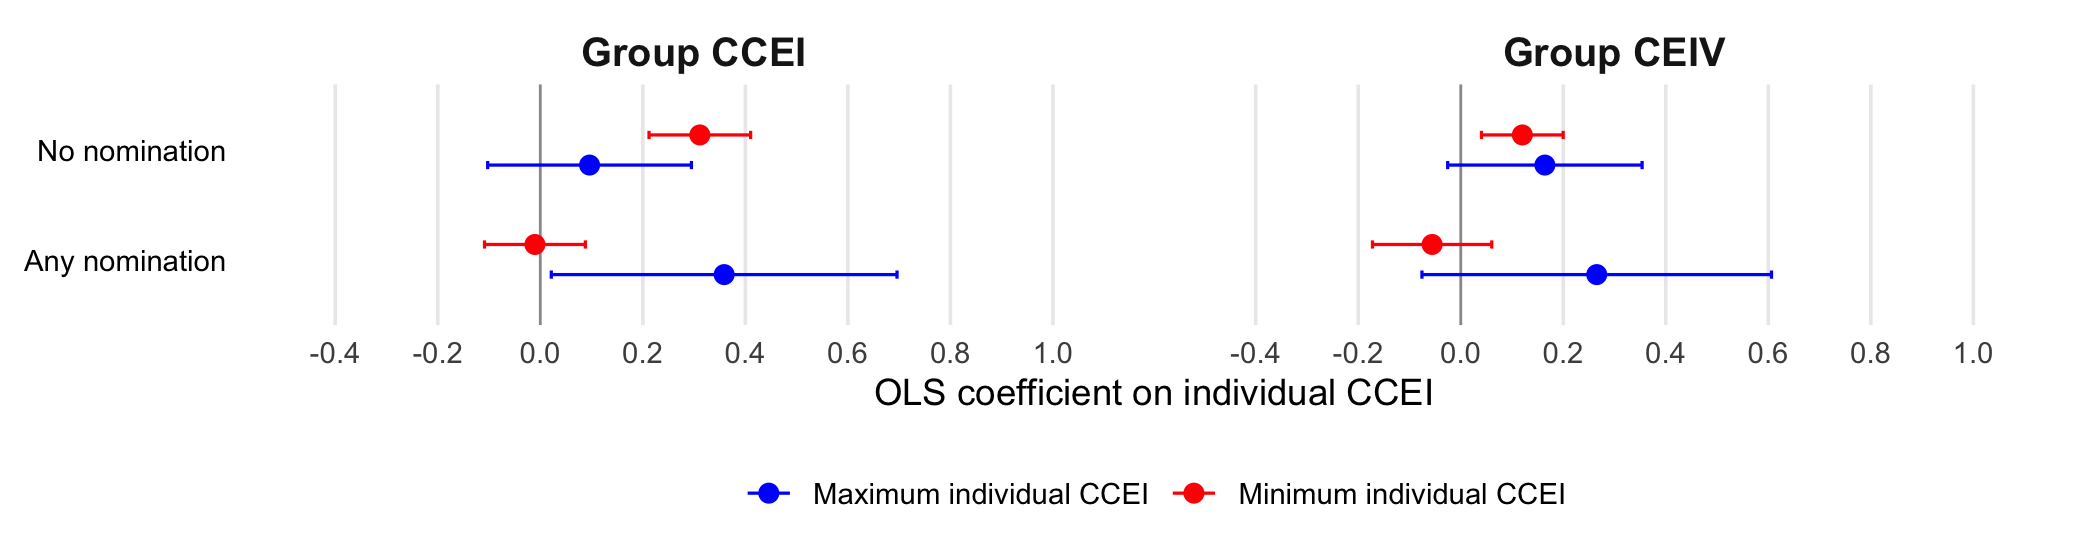
\includegraphics[width=\textwidth]{friend_any_coefficients.png}\end{center}
\begin{center}\begin{tabular}{lrrrrrr}\toprule
Sample & Fitted $N$ & Classes & CCEI: maximum & CCEI: minimum & CEIV: maximum & CEIV: minimum\\\midrule
Eligible pooled reference & 1304 & 64 & 0.131 (0.095) & 0.235 (0.045) & 0.176 (0.094) & 0.086 (0.035)\\
No nomination & 912 & 64 & 0.096 (0.099) & 0.311 (0.050) & 0.164 (0.095) & 0.120 (0.040)\\
Any nomination & 389 & 59 & 0.359 (0.168) & -0.010 (0.049) & 0.265 (0.170) & -0.056 (0.058)\\
\bottomrule\end{tabular}\end{center}
\begin{center}\begin{tabular}{llrrr}\toprule
Higher minus lower group & Individual CCEI & $\Delta$ group CCEI ($p$) & $\Delta$ CEIV ($p$) & $\Delta$(CCEI--CEIV) ($p$)\\\midrule
Higher minus lower & Minimum & -0.322 ($<0.001$) & -0.176 (0.018) & -0.146 (0.002)\\
Higher minus lower & Maximum & 0.263 (0.156) & 0.101 (0.587) & 0.161 (0.211)\\
\addlinespace\multicolumn{5}{l}{\textit{Wave-fixed-effects check: minimum CCEI}}\\
Higher minus lower & Minimum & -0.332 ($<0.001$) & -0.180 (0.015) & -0.152 (0.001)\\
\bottomrule\end{tabular}\end{center}
\textbf{Reading the pattern.} The minimum-CCEI slope is near zero among pairs with any nomination, compared with positive slopes among pairs with no nomination. The decline is larger for group CCEI than CEIV in this pooled friendship specification, including after adding wave controls. This is opposite to the predicted stronger minimum-CCEI association under easier communication.
\textit{Support check:} Mean minimum individual CCEI by subgroup: 0.856, 0.869; share of group CCEI equal to one: 43.9\%, 48.2\%. These describe eligible samples before singleton exclusions.
\textit{Notes:} Class-clustered SEs are in parentheses; 95\% intervals are plotted. Differences use pooled OLS fully interacting subgroup membership with both CCEIs, all controls, and class effects, accounting for shared classes. Pooled references use eligible samples; separate fits drop observations in singleton classes. Eligible counts are in the introduction; fitted counts are in the table.
\end{document}
